\chapter{Testing}

\section{Test setup}
Datasets

Using the Gnu Scientific Library taus random number generator, using a predefined seed,
30 million random strings were generated. This method was chosen to obtain a uniformly distributed
data on a larger scale, which is 
%GSL\_RNG\_SEED=110604190045 GSL\_RNG\_TYPE=taus /usr/bin/time -v ./tests/bin/seq/seq\_map > map\_30M.log 2>&1 
\begin{table}[h!]
    \centering
    \begin{tabular}[here]{l l l l l l}
        \hline
        Dataset    & Distinct   & Strings      & Avg     & Size (MB)& Size (MB)\\
                   &            &              & length  & distinct & total    \\\hline
        30M Random & 29,990,518 & 30,000,000   & 9.00    & 228.84   & 270.00\\
        Shakespeare&  31,229    & 340,039      & 5.56    & 0.21     & 18.91\\
        Newsgroups & 463,302    & 6,046,538    & 7.63    & 8.19     & 44.00\\
        \hline
    \end{tabular}
    \caption{Characteristics of the datasets used for insertions and self-search.}
    \label{tab:datasets}
\end{table}


The tests will be run on three different setups, to determine the impact of
increased parallelism, by utilizing 2, 4 and 8 cores respectively.

\begin{table}[h!]
    \centering
    \begin{tabular}[here]{ l l l l }
        \hline
                  & Intel \\\cline{2-4}
                  & Core 2 Duo T9300 & Core i7-950  & Xeon E5420 \\ \hline
        Abbrevation & C2D & i7 & Xeon \\ 
        CPU speed   & 2.50 GHz & 3.06 GHz & 2.50 GHz \\
        No. CPUs    & 1 & 1 & 2 \\
        Phys. Cores & 2 & 4 & 8 \\
        Virt. Cores & 0 & 4 & 0 \\
        L1/L2/L3 size(kB) & 64/6.144 & 128/1024/8.192 & 128/12.288\\
        L1/L2 cacheline(B) & 64/64 & 64/64 & 64/64\\
        %TLB entries & \\
        Memory (MB) & 4,096 & 8,192 & 32,768 \\
        Memory type & DDR2 800 & DDR3 1333 & DDR2 800 \\a
        Memory channels & 2 & 3 & 2 \\
        %Memory latency  & 
        Linux Kernel    & 2.6.38 & 2.6.38 & 2.6.36 \\
        Processor type  & 64-bit & 64-bit & 64-bit \\\hline
    \end{tabular}
    \caption{Characteristics of the used testing machines.}
    \label{tab:cpucpecs}
\end{table}

The Core 2 Duo machine is a Dell Laptop, chosen for its dual-core CPU.
The Xeon machine is a server workstation at DIKU, with two Xeon E5420 CPUs,
but is shared with many other students, which means that the workload
under testing was not under our control. The i7 machine was used for its
quad-core cpu, and with hyperthreading showing up as 8 cores, where 4 of them
are virtual, provides an interesting comparison with the Xeon machine, which
has 8 physical cores. The i7 machine was used for primary testing.

The tests themselves are run by running 10 iterations of the dataset, while randomizing
the order of the reference container, and thereby the search and insertion order
between every iteration, as well as between insertion and searching.


\section{Sequential tests}
For assessing the relative performances under a sequential environment, first a
baseline measurement of the {\keyword STL::Map} structure is made, on each of
the test machines.

\subsection{Uniformly distributed data}
Basic MAP result using the 30M dataset.

\begin{table}[h!]
    \centering
    \begin{tabular}[here]{ l l l }
        \hline
        Machine   & Insertion time & Self-search time  \\\hline
        C2D       & NA             & NA                \\\hline
        i7        & 112.74         & 110.45            \\\hline
        Xeon      & 231.33         & 231.56            \\\hline 
    \end{tabular}
    \caption{Base results for the STL::Map container, using the 30M random strings set.}
    \label{tab:maptimes}
\end{table}

Here, the primary difference of the machines lies in the amount of memory
available. Since the structure uses more than 4500 MB with the chosen dataset,
the Core2Duo setup uses paging to obtain the needed memory, and as such incurs
a huge performance hit when compared to the other two.

To verify this, Valgrind was run with the Massif heap profiler
[\pageref{fig:Massif_map_30m}], showing an allocation size of 434MB. Assuming
linear scaling, this is slightly lower than the observed 4450MB. Massif and
valgrind was unable to run on the full 30M set, because of added memory
overhead.
\begin{landscape}
    \begin{figure*}[h]
        \subfloat[Insert]{
            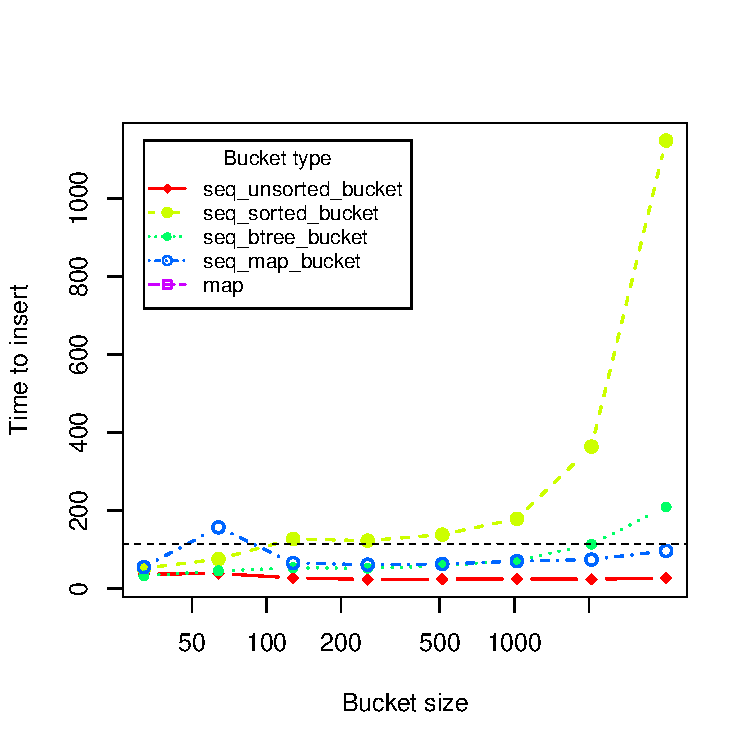
\includegraphics[width=1.0\textwidth]{plots/i7_30m_insert}
        }
        \subfloat[Search]{
            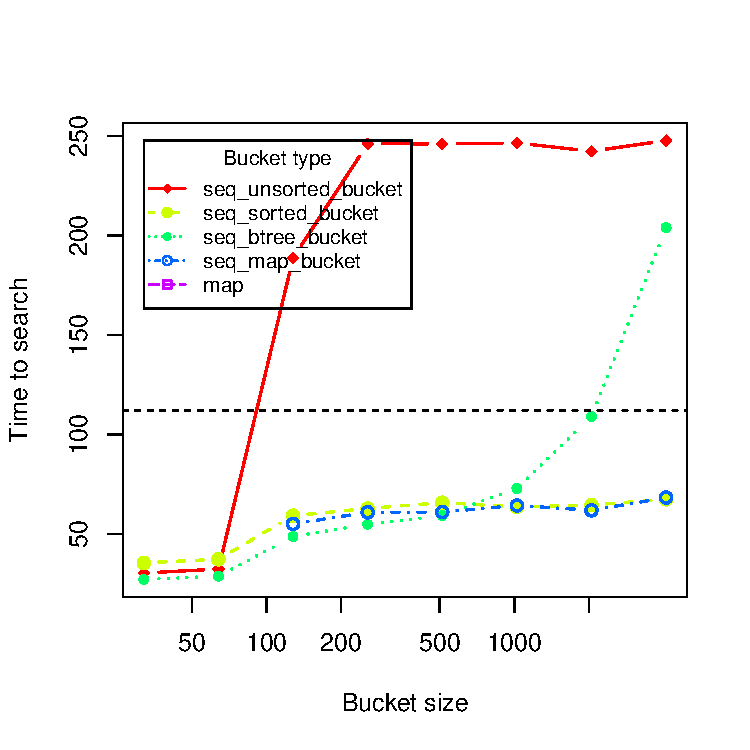
\includegraphics[width=1.0\textwidth]{plots/i7_30m_search}
        }
        \caption{Scaling of insertion and self-search times using the 30M Random
        dataset, with varying bucket sizes from 32 to 4096. The {\keyword map} time
        is shown for reference as a dotted line.}
        \label{fig:seq_30m}
    \end{figure*}
\end{landscape}

The expected constant-time insertion into unsorted arrays is evident, showing
an insertion time of $24$ to $38$ seconds.
The {\keyword map} bucket scales second best with larger bucket sizes, but
shows a large jump in memory use when compared to the other buckets, with smaller
bucket sizes. This is mainly attributed to large space overhead, from the
lookup tables, which becomes neglectible as the bucket count decreases.

\begin{table}[h]
    \centering
    \begin{tabular}[here]{ l l l }
        \hline
        Bucketsize& Node count  & Bucket count  \\\hline
        32        &  254,080    & 13,408,608  \\
        64        &  254,080    & 13,408,608  \\
        128       &  58,396     & 3,225,230   \\
        256       &  4033       & 250,047     \\
        \vdots    &  \vdots     & \vdots      \\
        4096      &  4033       & 250,047     \\\hline 
    \end{tabular}
    \caption{Bucket and node counts for the various bucket sizes using the
        30M dataset.}
    \label{tab:bncounts_30M}
\end{table}

\begin{figure}[!h]
    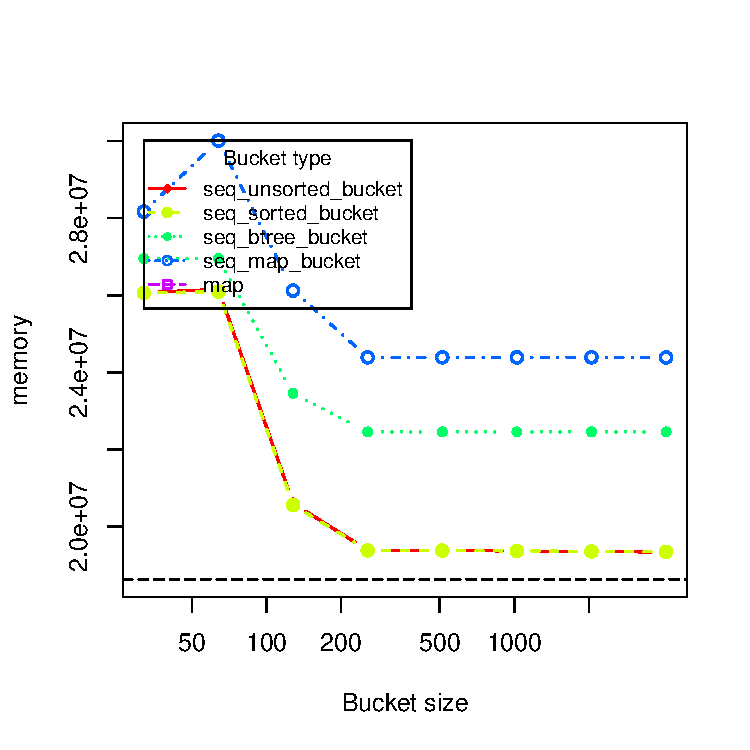
\includegraphics[width=1.0\textwidth]{plots/i7_30m_memory}
    \label{fig:memory_30m}
    \caption{Memory consumption (Max resident set size) of different
    bucket types and sizes.}
\end{figure}

With the counts being the same for several of the sizes, the cause for increased insertion times
must be an increased cost of bursting of the cost of bursting.
The binary trees also take an impact on increased bucket sizes, which is
a 
increased emphasis on insertion order may create deep buckets, which
also shows slightly in the insertion phase.


\subsection{Shakespeare dataset}
The shakespeare dataset is chosen for its real-world character distribution, and will
therefore present a good test-case for dictionary use of the structure.

\begin{table}[h]
    \centering
    \begin{tabular}[here]{ l l l }
        \hline
        Bucketsize&  Node count & Bucket count\\\hline
        32        &  4,511      & 12,396      \\
        64        &  2,565      & 9,155       \\ 
        128       &  1,372      & 6,432       \\ 
        256       &  659        & 4,203       \\ 
        512       &  340        & 2,770       \\ 
        1024      &  155        & 1,750       \\ 
        2048      &  99         & 1,231       \\ 
        4096      &  44         & 580         \\ \hline
    \end{tabular}
    \caption{Bucket and node counts for the various bucket sizes using the Shakespeare
        dataset.}
    \label{tab:bncounts_shakespeare}
\end{table}

\subsection{Newsgroups dataset}
w00h!



\section{Parallel scaling}

Locking improvement: per-node lock.

foreach buckettype: vary sizes, locking method,
                    number of threads, number of cores

Amdahls law.

False sharing!! [REF] 


\subsection{Datasets}
The Shakespeare dataset requires a threadsafe multiple-readers structure to
allow the threads to concurrently extract words from the dataset after first
reading them into memory.

I have therefore implemented a simple CREW (concurrent read exclusive write)
vector for this purpose. The base performance of this is a memory consumption
of 8 times the word count bytes from pointers, plus the size of the dataset
itself. (Overhead in std::string?)
\begin{landscape}
    % i7 !!
    \begin{figure}[!h]
        \subfloat[Insertion time] {
            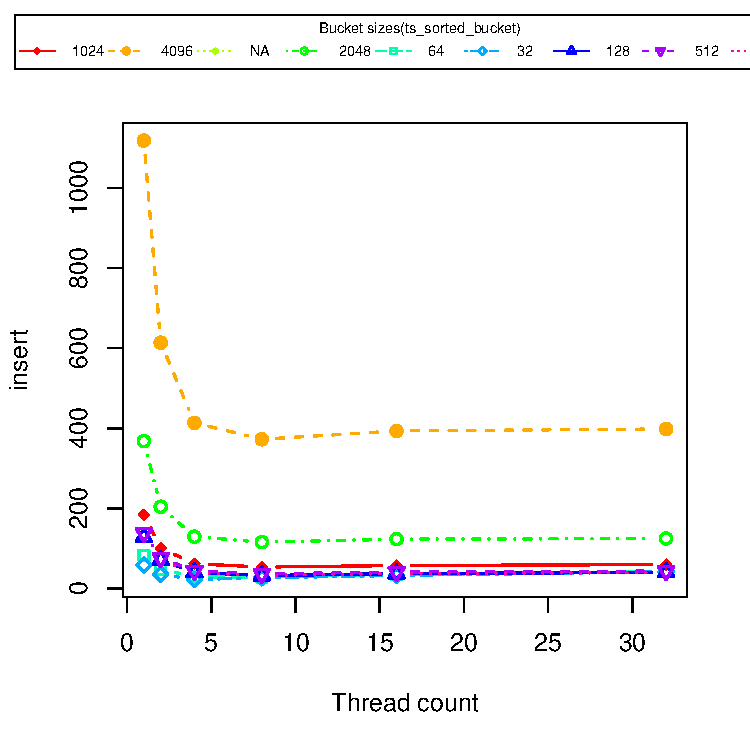
\includegraphics[width=1.0\textwidth]{plots/i7/plot_0_ts_sorted_bucketinsert}
        }
        \subfloat[Search] {
            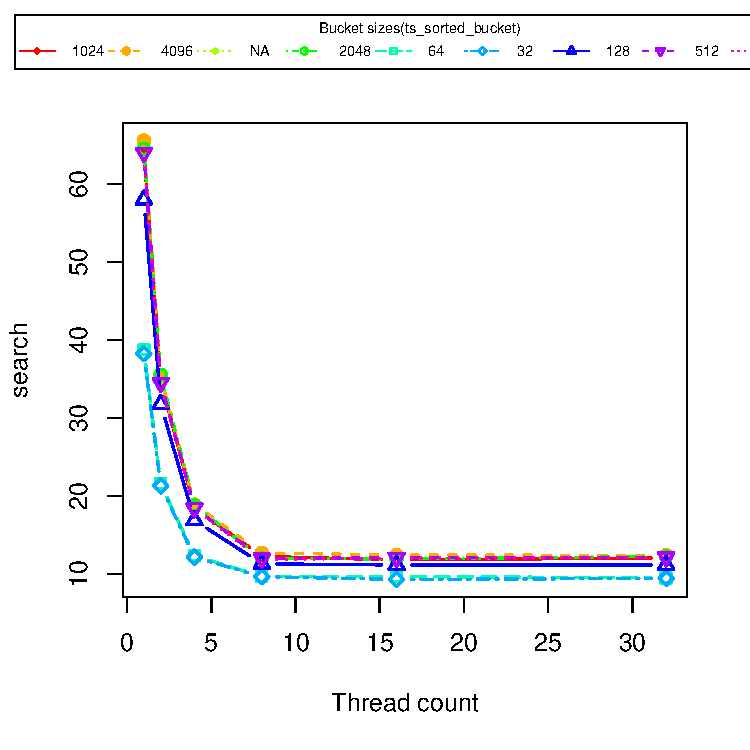
\includegraphics[width=1.0\textwidth]{plots/i7/plot_0_ts_sorted_bucketsearch}
        }
        \label{fig:ts_i7_30m_sorted}
        \caption{Multithreaded scaling of the sorted dynamic array bucket with varying sizes on the
        i7 machine (4+4 cores). Testing done with the 30M dataset.}
    \end{figure}
    \begin{figure}[!h]
        \subfloat[Insertion time] {
            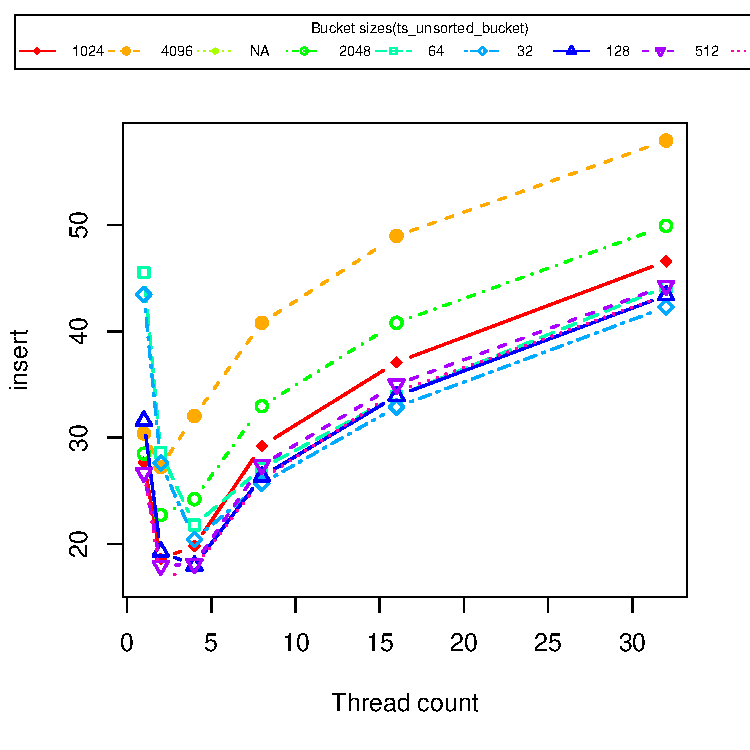
\includegraphics[width=1.0\textwidth]{plots/i7/plot_0_ts_unsorted_bucketinsert}
        }
        \subfloat[Search] {
            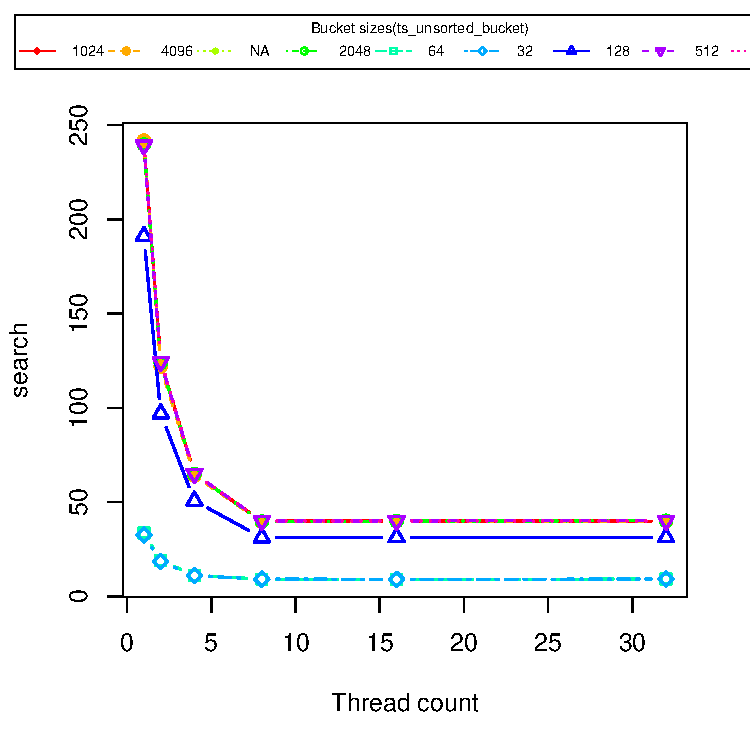
\includegraphics[width=1.0\textwidth]{plots/i7/plot_0_ts_unsorted_bucketsearch}
        }
        \label{fig:ts_i7_30m_unsorted}
        \caption{Multithreaded scaling of the unsorted dynamic array bucket with varying sizes on the
        i7 machine (4+4 cores). Testing done with the 30M dataset.}
    \end{figure}
    \begin{figure}[!h]
        \subfloat[Insertion time] {
            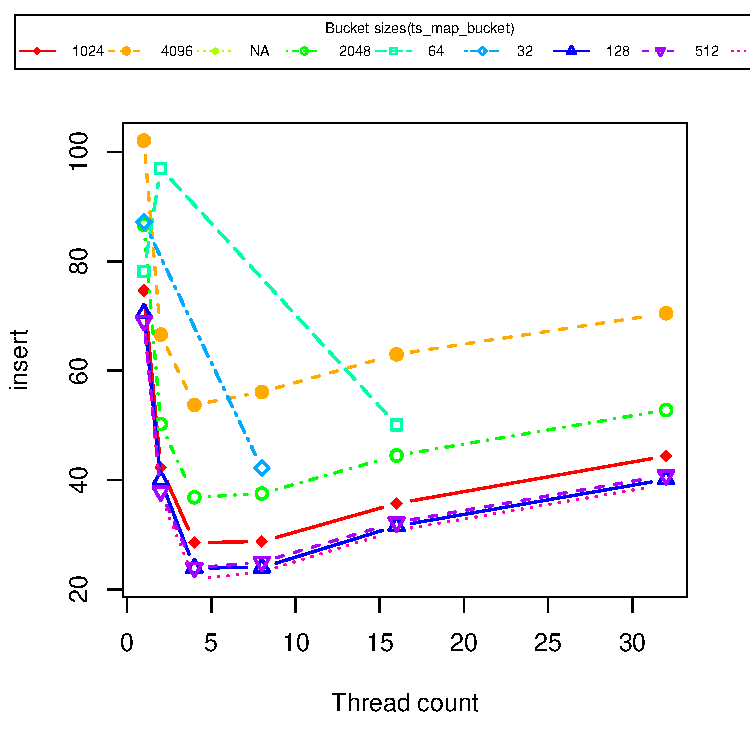
\includegraphics[width=1.0\textwidth]{plots/i7/plot_0_ts_map_bucketinsert}
        }
        \subfloat[Search] {
            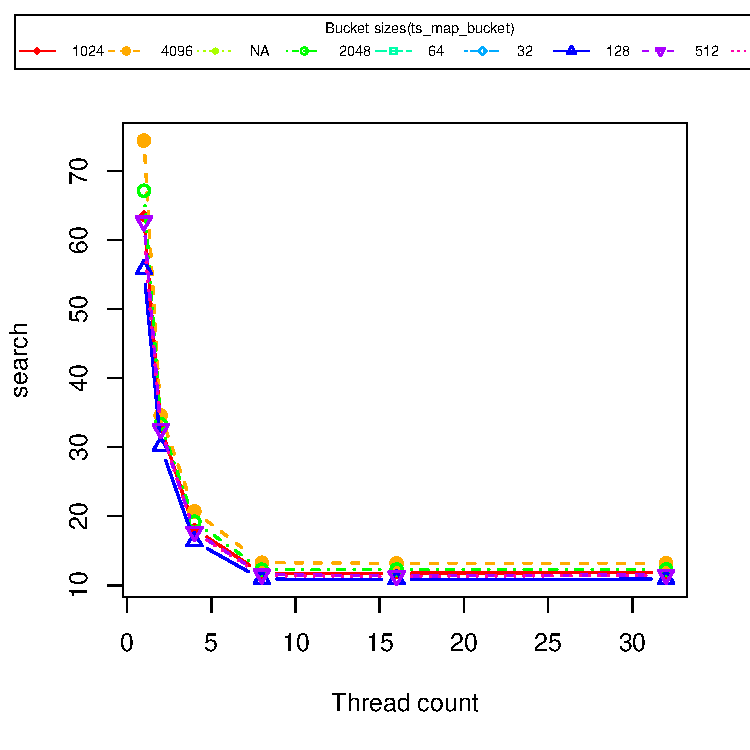
\includegraphics[width=1.0\textwidth]{plots/i7/plot_0_ts_map_bucketsearch}
        }
        \label{fig:ts_i7_30m_map}
        \caption{Multithreaded scaling of the STL::Map bucket with varying sizes on the
        i7 machine (4+4 cores). Testing done with the 30M dataset.}
    \end{figure}
    \begin{figure}[!h]
        \subfloat[Insertion time] {
            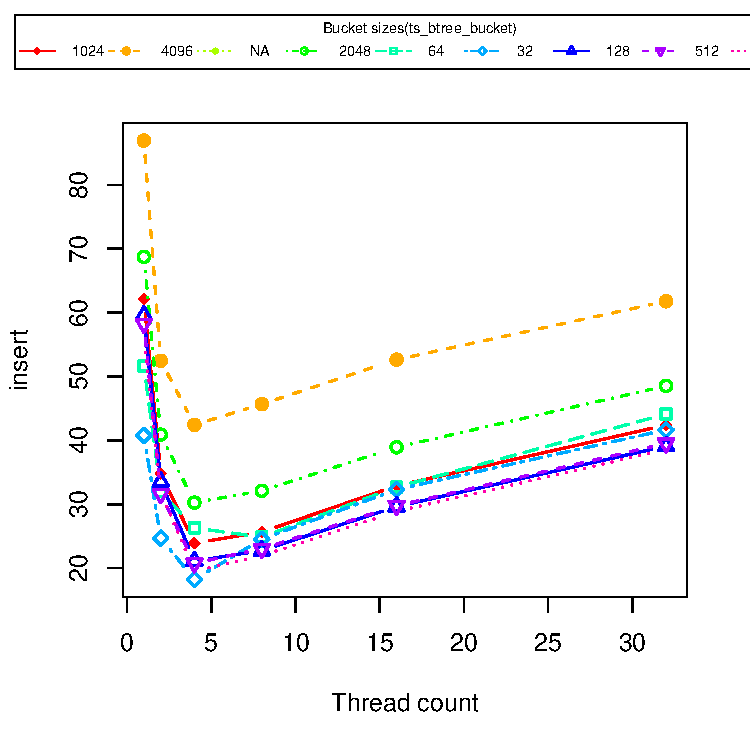
\includegraphics[width=1.0\textwidth]{plots/i7/plot_0_ts_btree_bucketinsert}
        }
        \subfloat[Search] {
            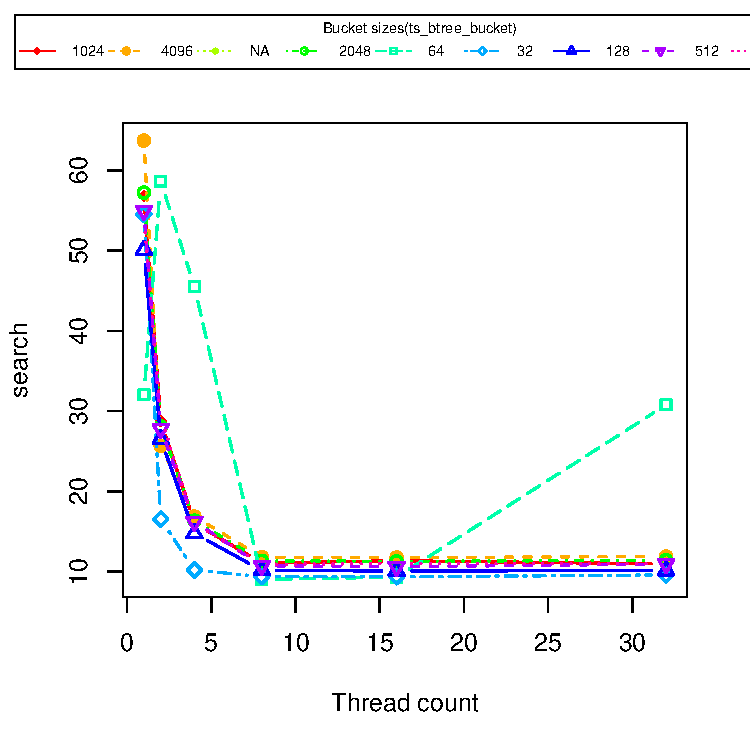
\includegraphics[width=1.0\textwidth]{plots/i7/plot_0_ts_btree_bucketsearch}
        }
        \label{fig:ts_i7_30m_btree}
        \caption{Multithreaded scaling of the binary tree bucket with varying sizes on the
        i7 machine (4+4 cores). Testing done with the 30M dataset.}
    \end{figure}
\end{landscape}

This is amazing!
YAY
w00h!

\begin{landscape}
    % c2d !!
    \begin{figure}[!h]
        \subfloat[Insertion time] {
            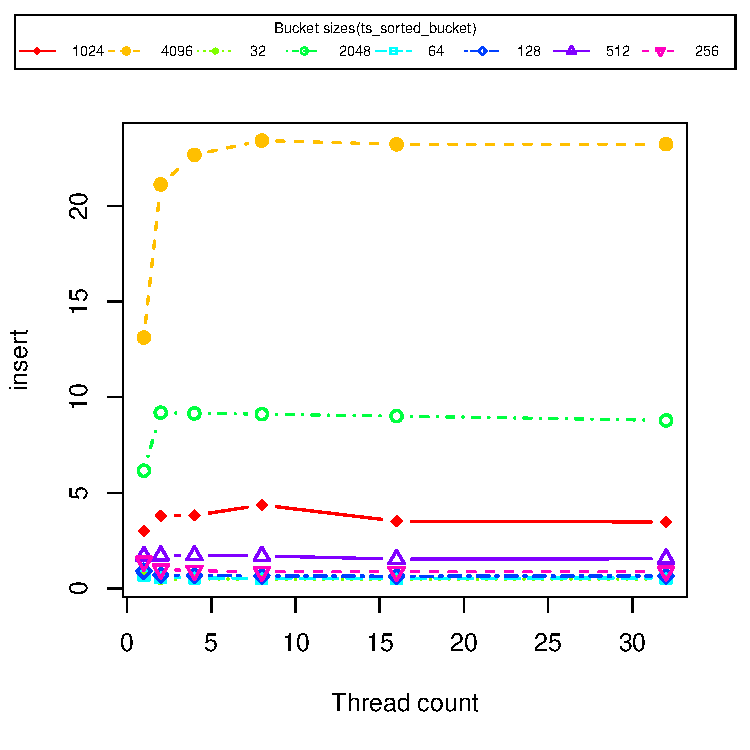
\includegraphics[width=1.0\textwidth]{plots/c2d/plot_1_ts_sorted_bucketinsert}
        }
        \subfloat[Search] {
            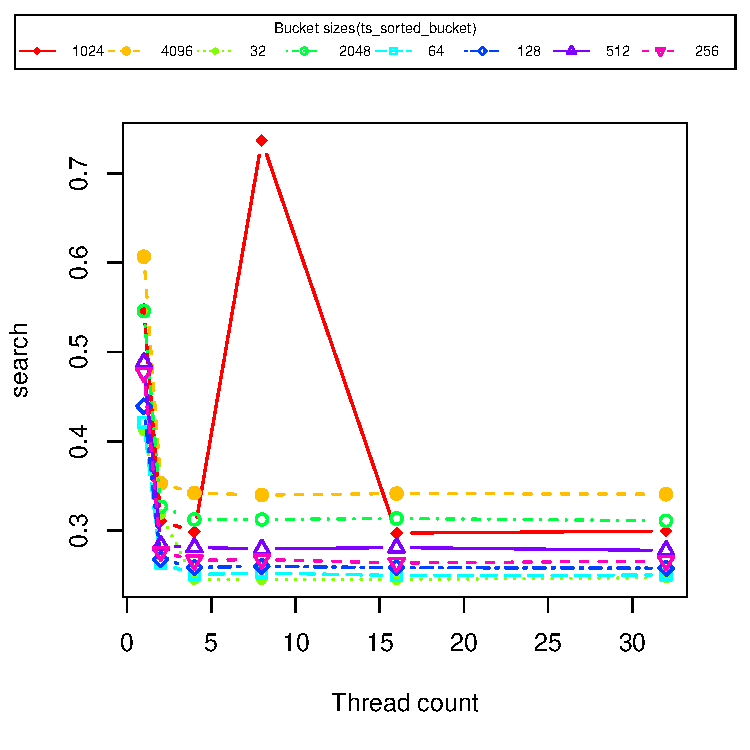
\includegraphics[width=1.0\textwidth]{plots/c2d/plot_1_ts_sorted_bucketsearch}
        }
        \label{fig:ts_c2d_shake_sorted}
        \caption{Multithreaded scaling of the sorted dynamic array bucket with varying sizes on the
        c2d machine (2 cores). Testing done with the shakespeare dataset.}
    \end{figure}
    \begin{figure}[!h]
        \subfloat[Insertion time] {
            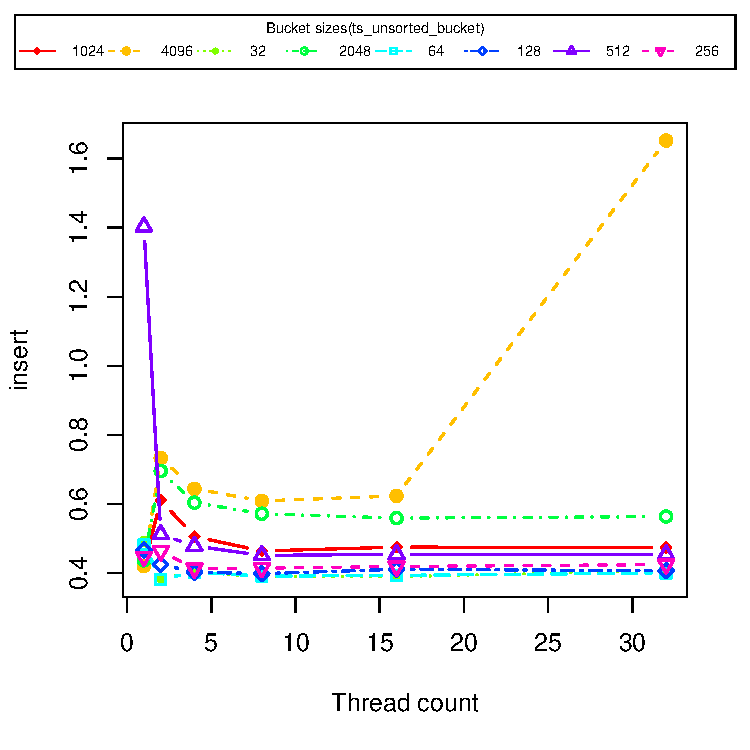
\includegraphics[width=1.0\textwidth]{plots/c2d/plot_1_ts_unsorted_bucketinsert}
        }
        \subfloat[Search] {
            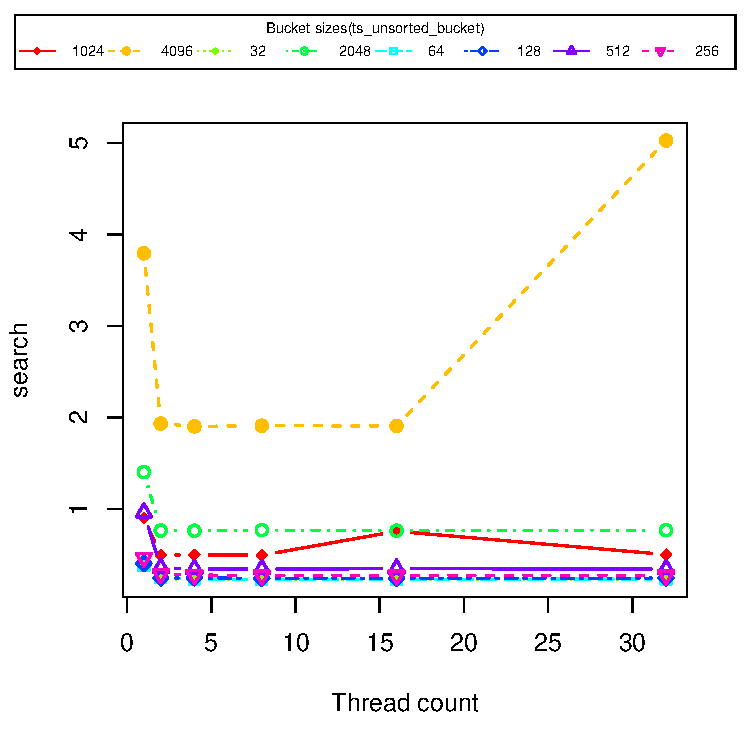
\includegraphics[width=1.0\textwidth]{plots/c2d/plot_1_ts_unsorted_bucketsearch}
        }
        \label{fig:ts_c2d_shake_unsorted}
        \caption{Multithreaded scaling of the unsorted dynamic array bucket with varying sizes on the
        c2d machine (2 cores). Testing done with the shakespeare dataset.}
    \end{figure}
    \begin{figure}[!h]
        \subfloat[Insertion time] {
            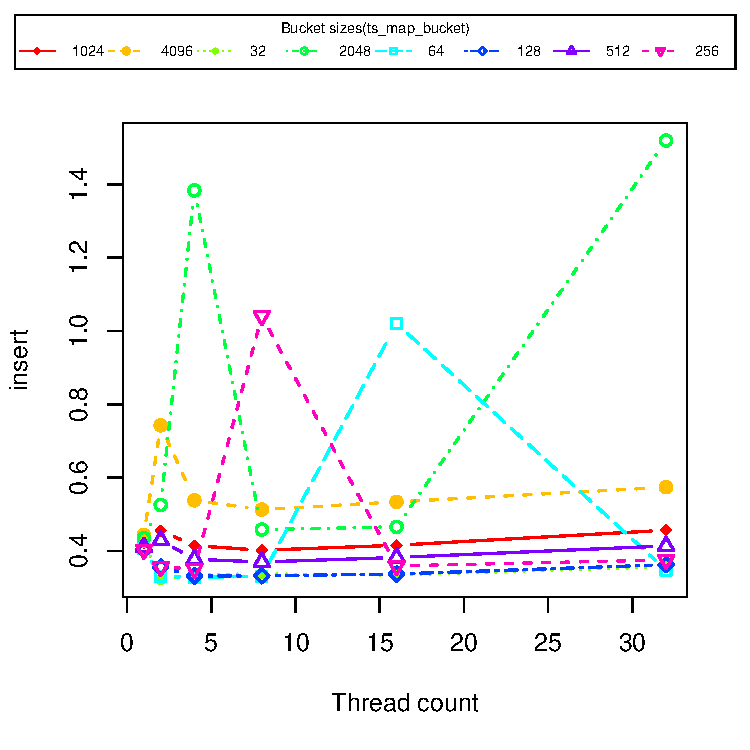
\includegraphics[width=1.0\textwidth]{plots/c2d/plot_1_ts_map_bucketinsert}
        }
        \subfloat[Search] {
            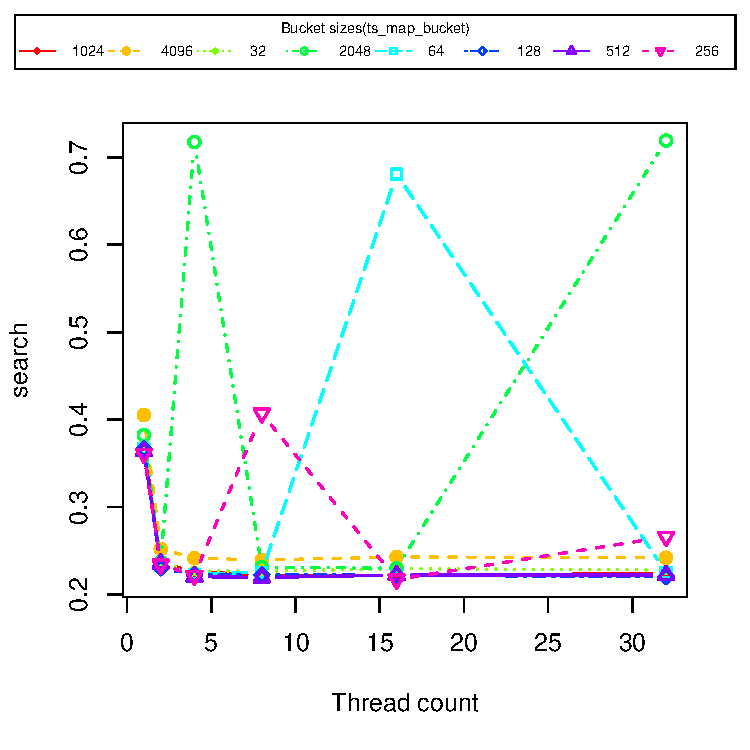
\includegraphics[width=1.0\textwidth]{plots/c2d/plot_1_ts_map_bucketsearch}
        }
        \label{fig:ts_c2d_shake_map}
        \caption{Multithreaded scaling of the STL::Map bucket with varying sizes on the
        c2d machine (2 cores). Testing done with the shakespeare dataset.}
    \end{figure}
    \begin{figure}[!h]
        \subfloat[Insertion time] {
            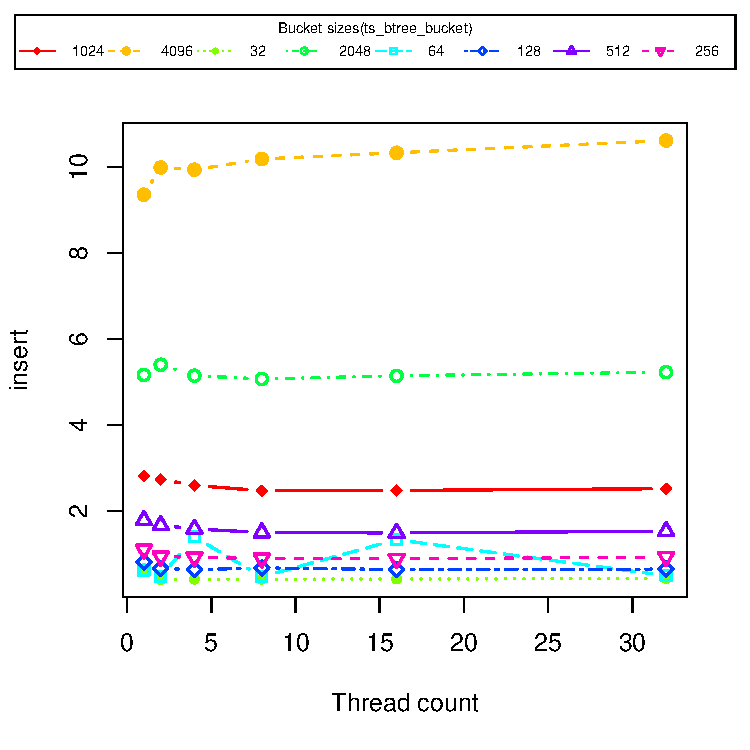
\includegraphics[width=1.0\textwidth]{plots/c2d/plot_1_ts_btree_bucketinsert}
        }
        \subfloat[Search] {
            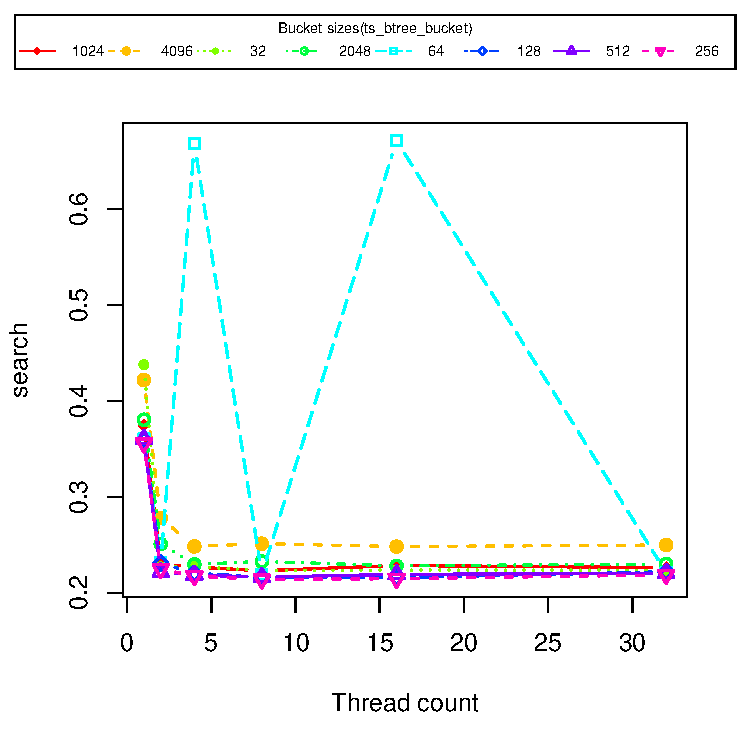
\includegraphics[width=1.0\textwidth]{plots/c2d/plot_1_ts_btree_bucketsearch}
        }
        \label{fig:ts_c2d_shake_btree}
        \caption{Multithreaded scaling of the binary tree bucket with varying sizes on the
        c2d machine (2 cores). Testing done with the shakespeare dataset.}
    \end{figure}
    % i7 !!
    \begin{figure}[!h]
        \subfloat[Insertion time] {
            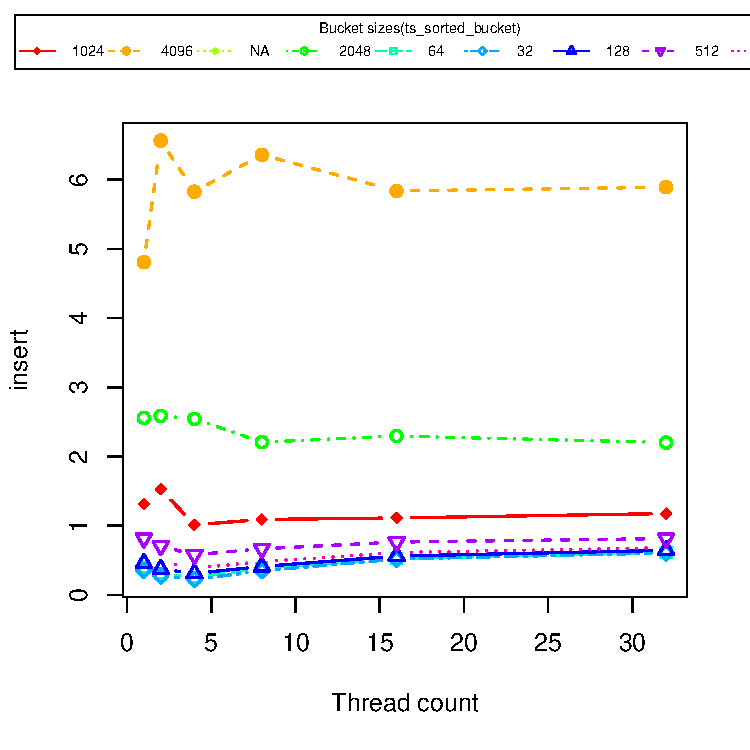
\includegraphics[width=1.0\textwidth]{plots/i7/plot_1_ts_sorted_bucketinsert}
        }
        \subfloat[Search] {
            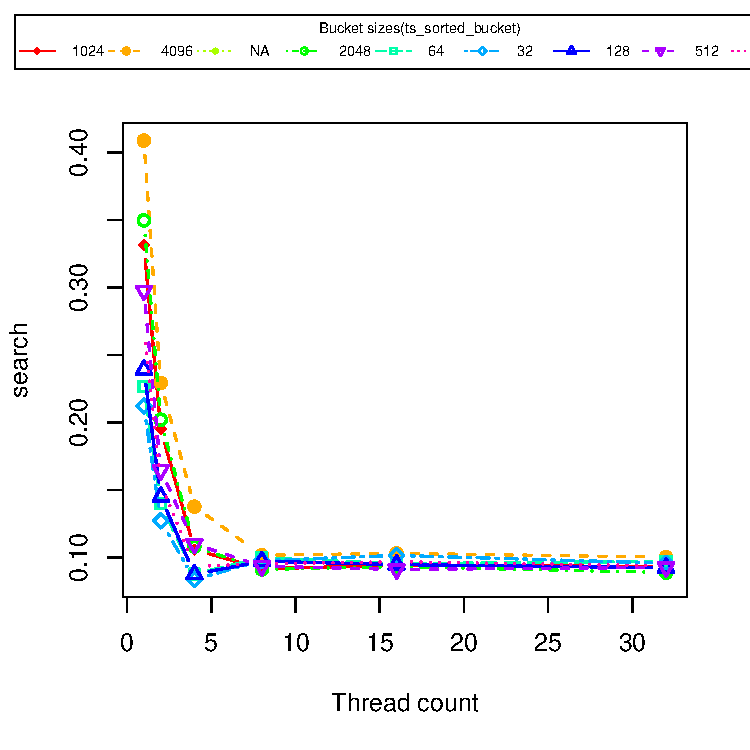
\includegraphics[width=1.0\textwidth]{plots/i7/plot_1_ts_sorted_bucketsearch}
        }
        \label{fig:ts_i7_shake_sorted}
        \caption{Multithreaded scaling of the sorted dynamic array bucket with varying sizes on the
        i7 machine (4+4 cores). Testing done with the shakespeare dataset.}
    \end{figure}
    \begin{figure}[!h]
        \subfloat[Insertion time] {
            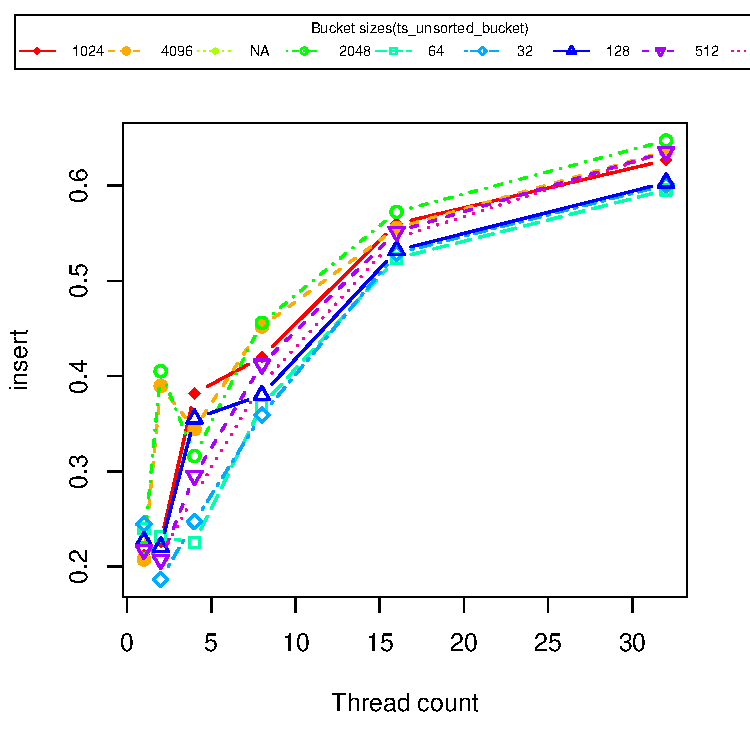
\includegraphics[width=1.0\textwidth]{plots/i7/plot_1_ts_unsorted_bucketinsert}
        }
        \subfloat[Search] {
            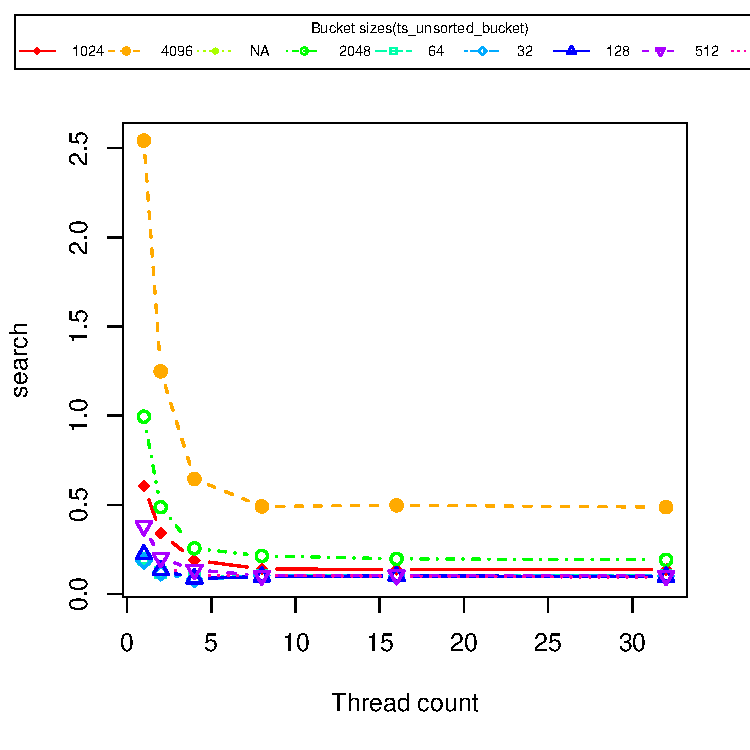
\includegraphics[width=1.0\textwidth]{plots/i7/plot_1_ts_unsorted_bucketsearch}
        }
        \label{fig:ts_i7_shake_unsorted}
        \caption{Multithreaded scaling of the unsorted dynamic array bucket with varying sizes on the
        i7 machine (4+4 cores). Testing done with the shakespeare dataset.}
    \end{figure}
    \begin{figure}[!h]
        \subfloat[Insertion time] {
            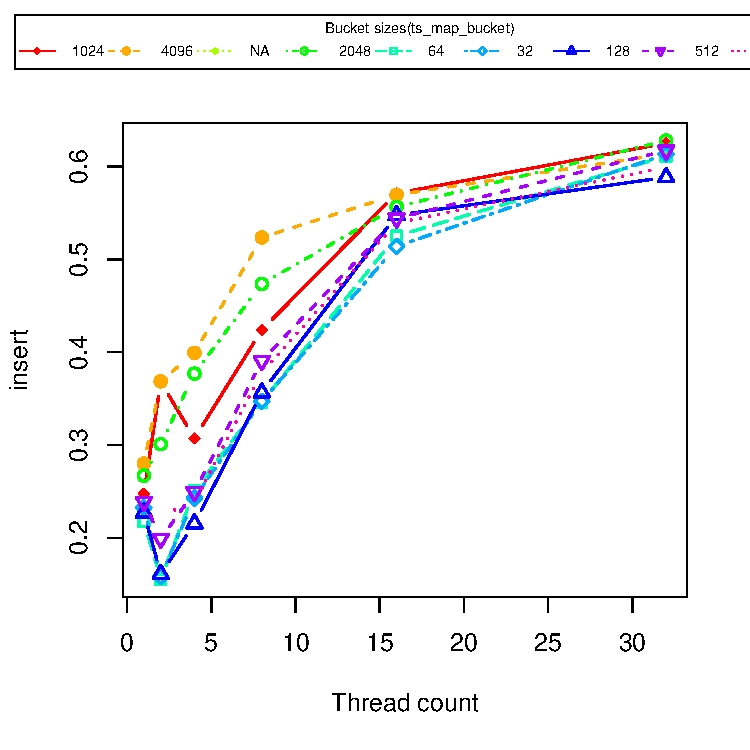
\includegraphics[width=1.0\textwidth]{plots/i7/plot_1_ts_map_bucketinsert}
        }
        \subfloat[Search] {
            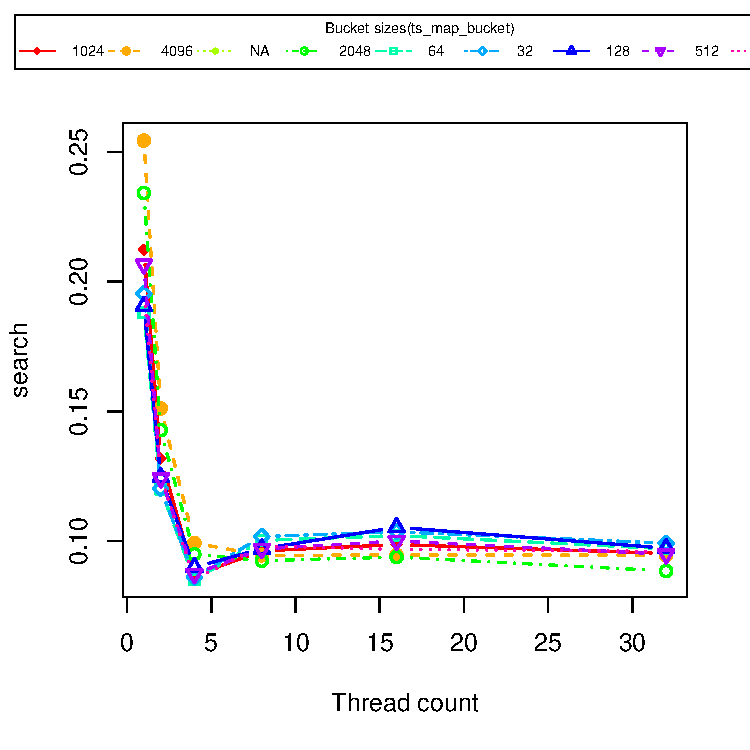
\includegraphics[width=1.0\textwidth]{plots/i7/plot_1_ts_map_bucketsearch}
        }
        \label{fig:ts_i7_shake_map}
        \caption{Multithreaded scaling of the STL::Map bucket with varying sizes on the
        i7 machine (4+4 cores). Testing done with the shakespeare dataset.}
    \end{figure}
    \begin{figure}[!h]
        \subfloat[Insertion time] {
            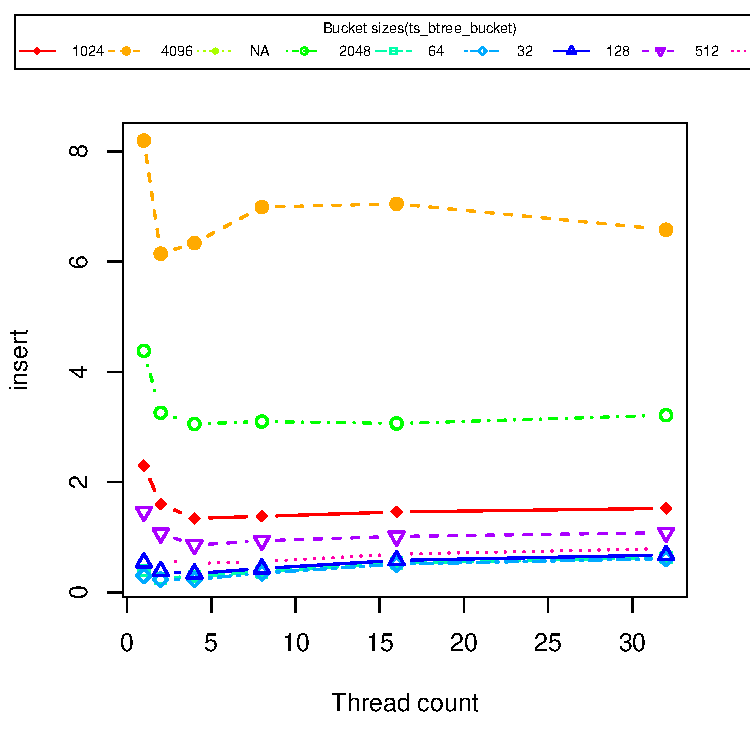
\includegraphics[width=1.0\textwidth]{plots/i7/plot_1_ts_btree_bucketinsert}
        }
        \subfloat[Search] {
            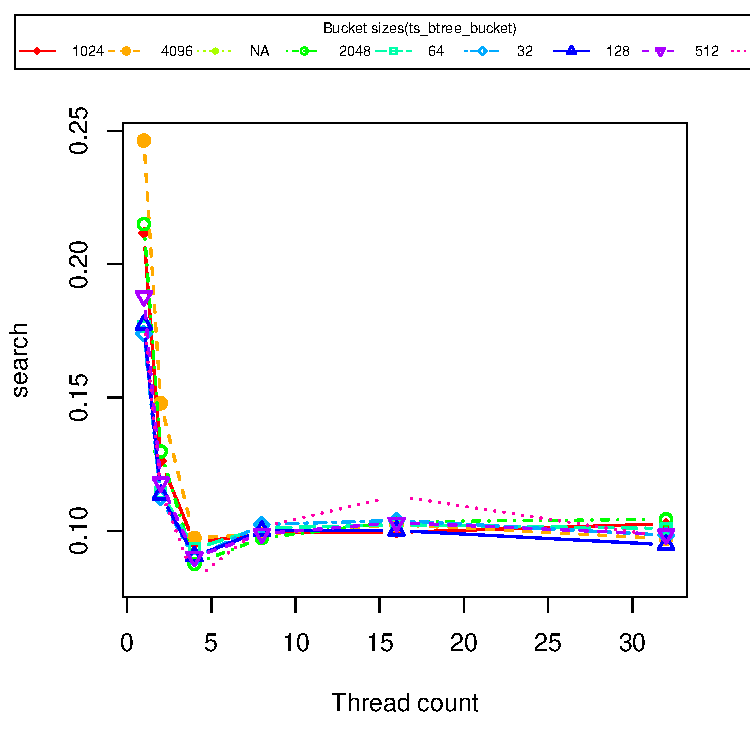
\includegraphics[width=1.0\textwidth]{plots/i7/plot_1_ts_btree_bucketsearch}
        }
        \label{fig:ts_i7_shake_btree}
        \caption{Multithreaded scaling of the binary tree bucket with varying sizes on the
        i7 machine (4+4 cores). Testing done with the shakespeare dataset.}
    \end{figure}
    % Xeon
    \begin{figure}[!h]
        \subfloat[Insertion time] {
            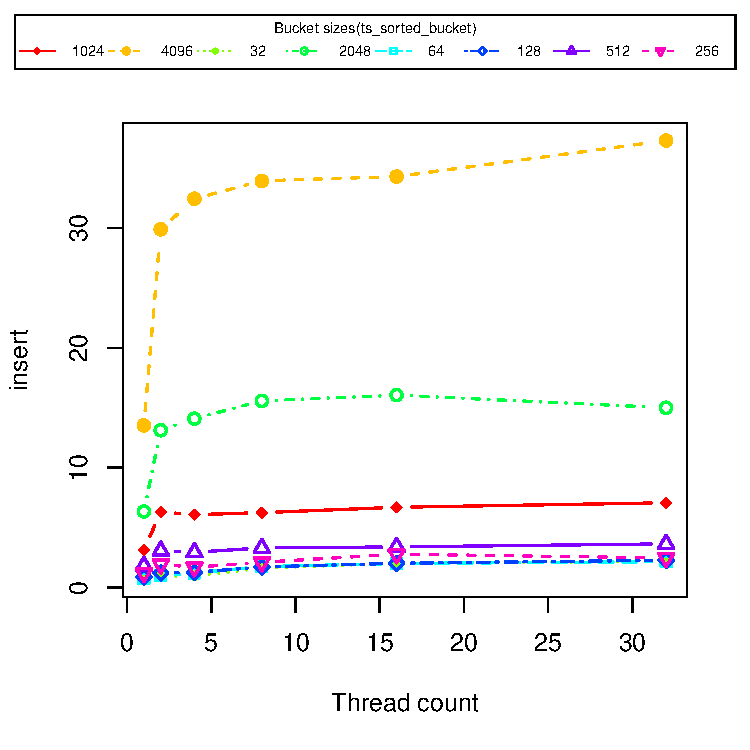
\includegraphics[width=1.0\textwidth]{plots/ask/plot_1_ts_sorted_bucketinsert}
        }
        \subfloat[Search] {
            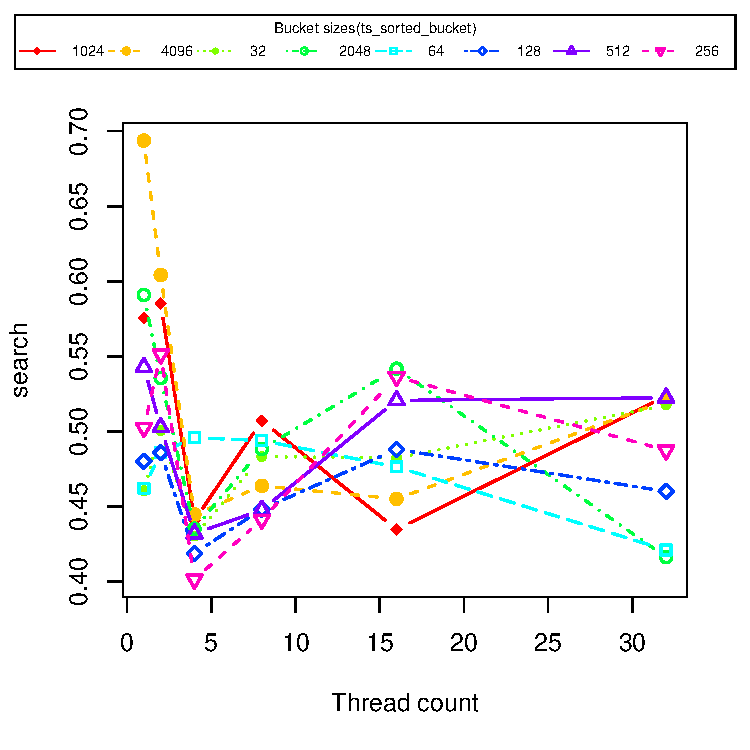
\includegraphics[width=1.0\textwidth]{plots/ask/plot_1_ts_sorted_bucketsearch}
        }
        \label{fig:ts_ask_i7_sorted}
        \caption{Multithreaded scaling of the sorted dynamic array bucket with varying sizes on the
        Xeon machine (8 cores). Testing done with the shakespeare dataset.}
    \end{figure}
    \begin{figure}[!h]
        \subfloat[Insertion time] {
            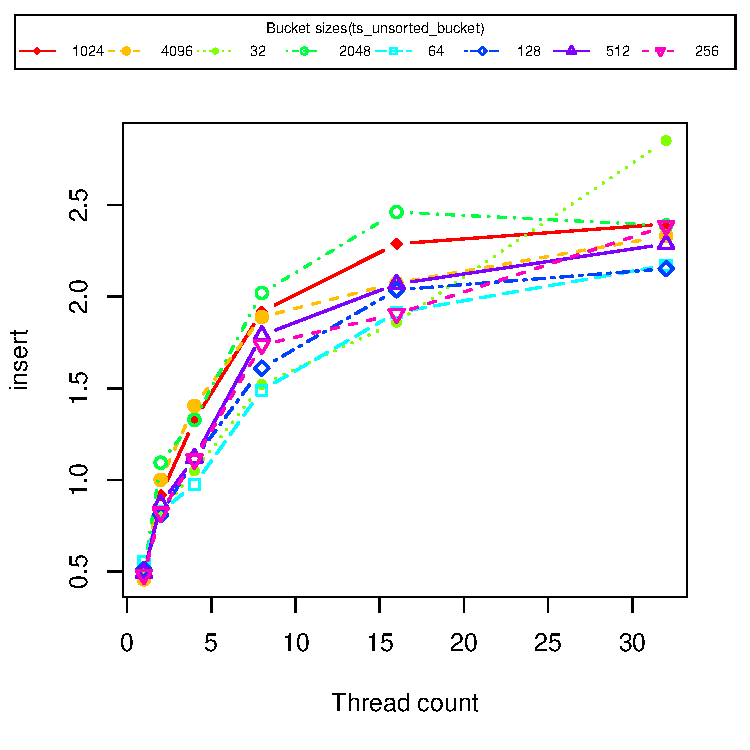
\includegraphics[width=1.0\textwidth]{plots/ask/plot_1_ts_unsorted_bucketinsert}
        }
        \subfloat[Search] {
            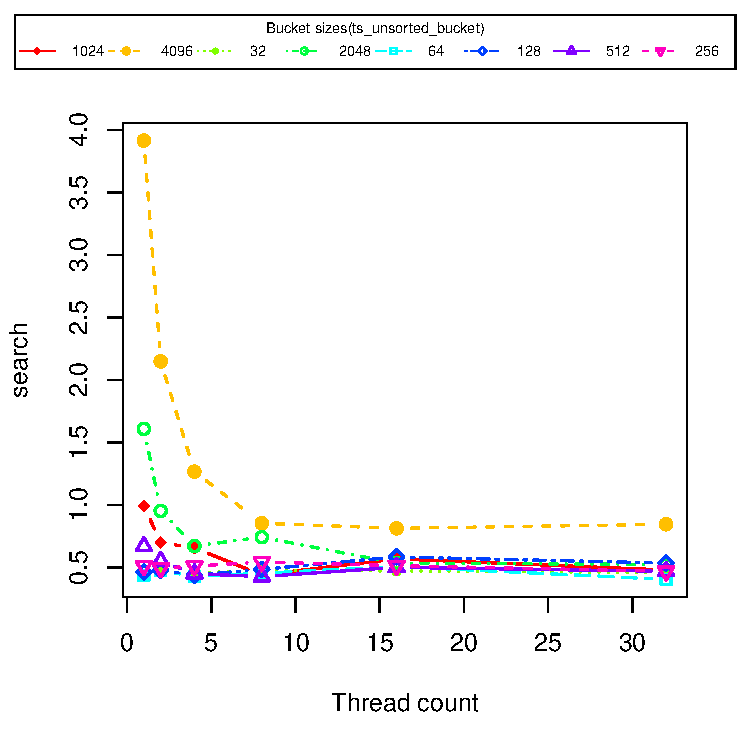
\includegraphics[width=1.0\textwidth]{plots/ask/plot_1_ts_unsorted_bucketsearch}
        }
        \label{fig:ts_ask_shake_unsorted}
        \caption{Multithreaded scaling of the unsorted dynamic array bucket with varying sizes on the
        Xeon machine (8 cores). Testing done with the shakespeare dataset.}
    \end{figure}
    \begin{figure}[!h]
        \subfloat[Insertion time] {
            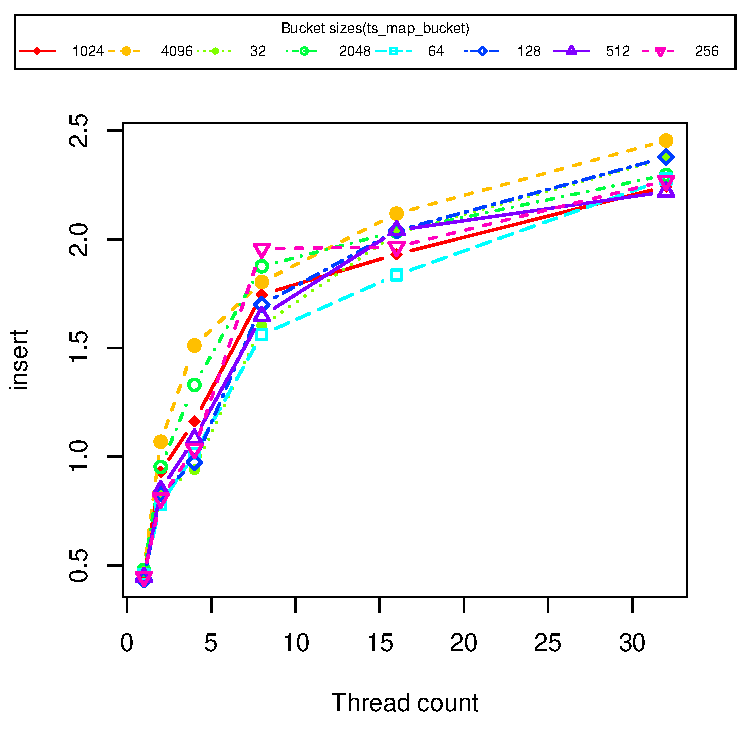
\includegraphics[width=1.0\textwidth]{plots/ask/plot_1_ts_map_bucketinsert}
        }
        \subfloat[Search] {
            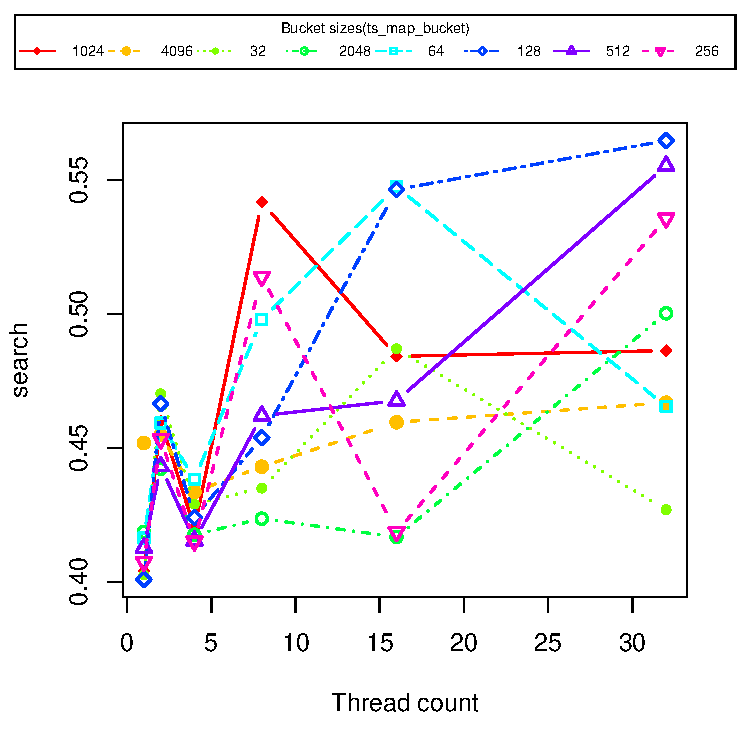
\includegraphics[width=1.0\textwidth]{plots/ask/plot_1_ts_map_bucketsearch}
        }
        \label{fig:ts_ask_shake_map}
        \caption{Multithreaded scaling of the STL::Map bucket with varying sizes on the
        Xeon machine (8 cores). Testing done with the shakespeare dataset.}
    \end{figure}
    \begin{figure}[!h]
        \subfloat[Insertion time] {
            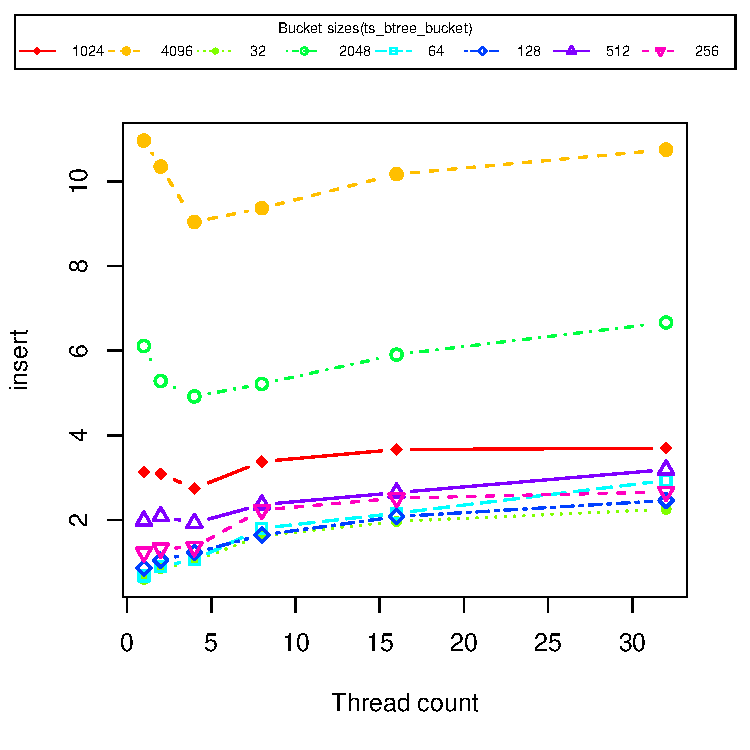
\includegraphics[width=1.0\textwidth]{plots/ask/plot_1_ts_btree_bucketinsert}
        }
        \subfloat[Search] {
            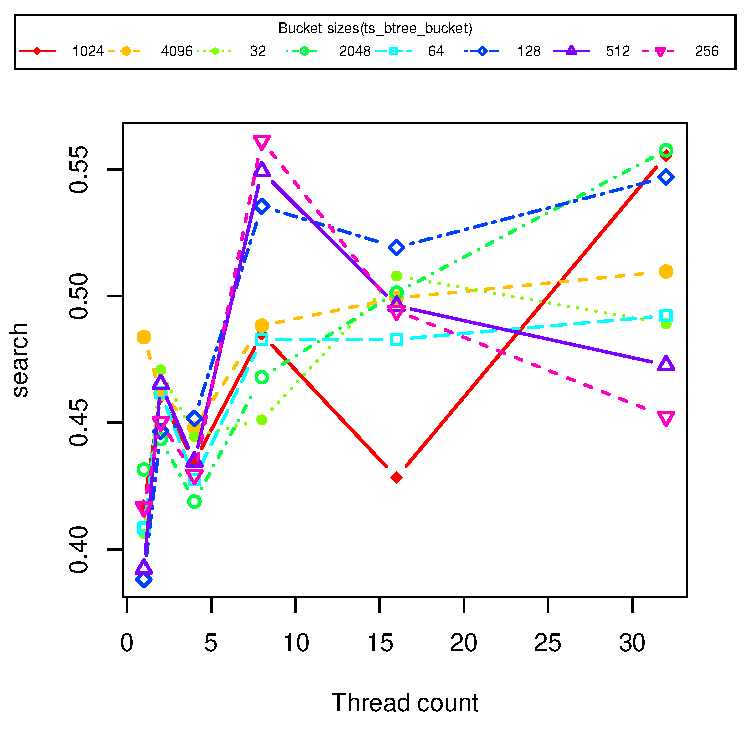
\includegraphics[width=1.0\textwidth]{plots/ask/plot_1_ts_btree_bucketsearch}
        }
        \label{fig:ts_ask_shake_btree}
        \caption{Multithreaded scaling of the binary tree bucket with varying sizes on the
        Xeon machine (8 cores). Testing done with the shakespeare dataset.}
    \end{figure}
\end{landscape}

These tests show a clear bottleneck already beginning to show at 2 cores for insertions, while
the concurrent locking on insertions allows full parallelism to the order of the number of cores
available. This is caused by the shallow trie, which is an issue due to node-level parallelism.

Due to sharing of the locks, that needs to be synchronized between caches, on an expensive
interconnect, the scaling is negative. That is, the overhead created by synchronization of
the node locks is greater than the gain in parallelism. The 



